% l = 8
\begin{figure}[htp]
\begin{center}
\subfloat{
\resizebox{8cm}{5cm}{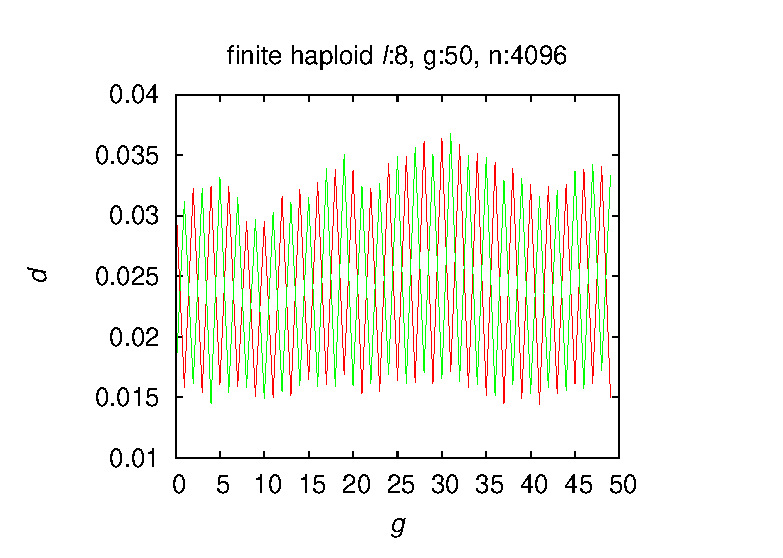
\includegraphics{figures/eps/osc/b8/n004096_osc_fin_hap.eps}}} \hspace{-3em}% 
\subfloat{
\resizebox{8cm}{5cm}{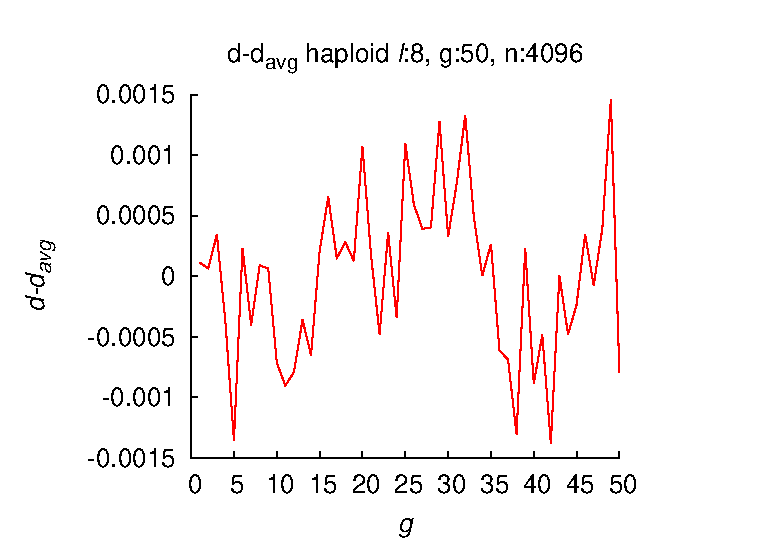
\includegraphics{figures/eps/osc/b8/n004096_osc_fin_hap_dist.eps}}} \vspace{-1em}  \hspace{-3em}% 

\end{center}
\begin{center}
\subfloat{
\resizebox{8cm}{5cm}{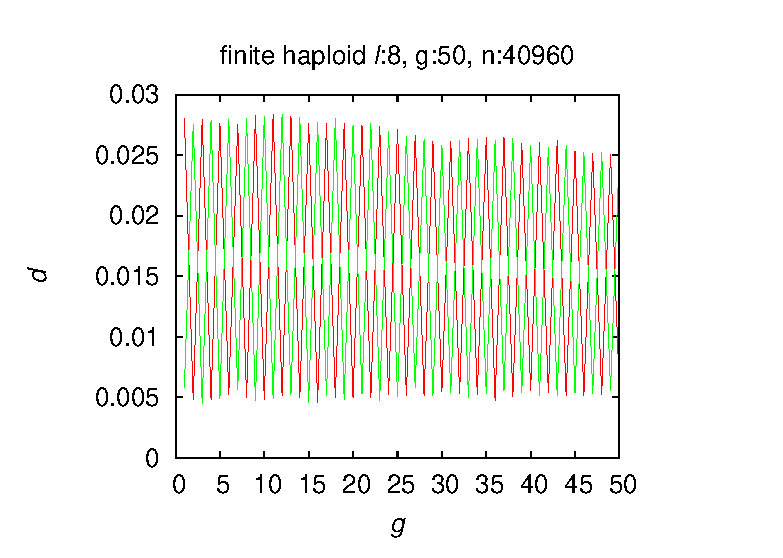
\includegraphics{figures/eps/osc/b8/n040960_osc_fin_hap.eps}}} \hspace{-3em}% 
\subfloat{
\resizebox{8cm}{5cm}{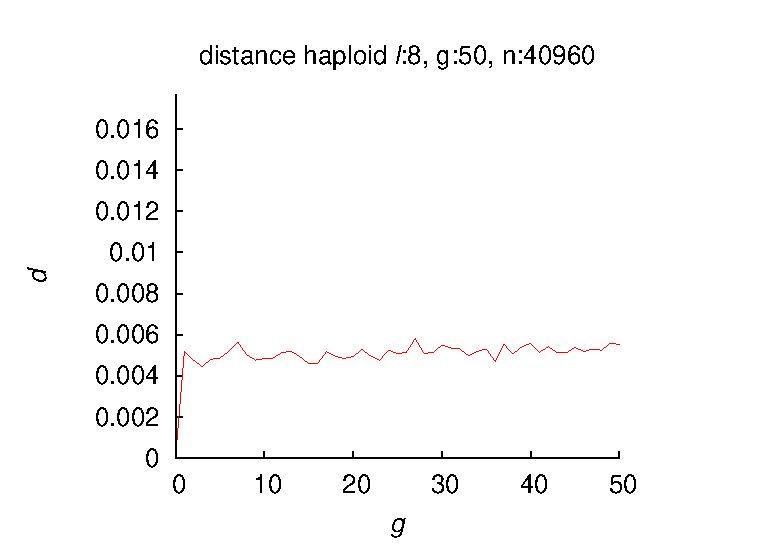
\includegraphics{figures/eps/osc/b8/n040960_osc_fin_hap_dist.eps}}} \vspace{-1em}  \hspace{-3em}% 
\end{center}

\begin{center}
\subfloat{
\resizebox{8cm}{5cm}{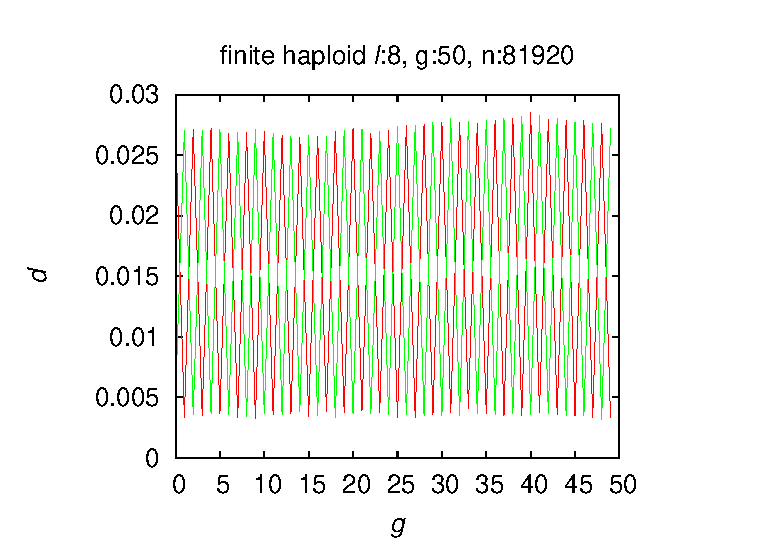
\includegraphics{figures/eps/osc/b8/n081920_osc_fin_hap.eps}}} \hspace{-3em}% 
\subfloat{
\resizebox{8cm}{5cm}{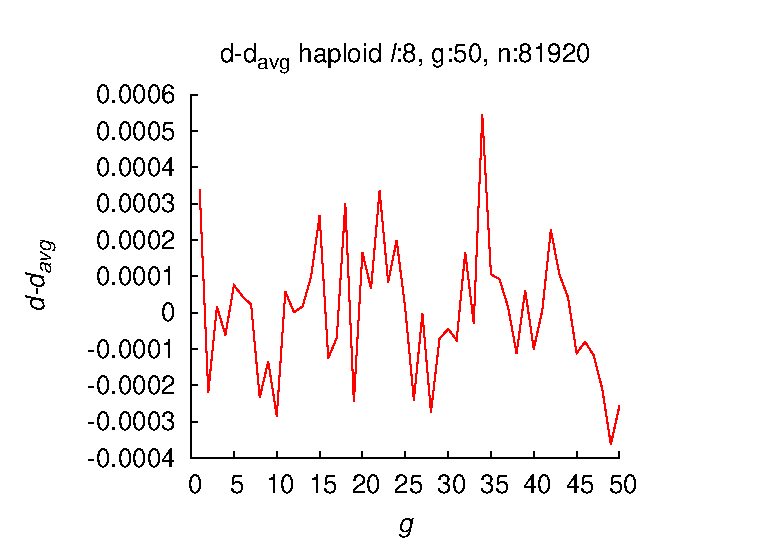
\includegraphics{figures/eps/osc/b8/n081920_osc_fin_hap_dist.eps}}} \vspace{-1em}  \hspace{-3em}% 
\end{center}


\begin{center}
\subfloat{
\resizebox{8cm}{5cm}{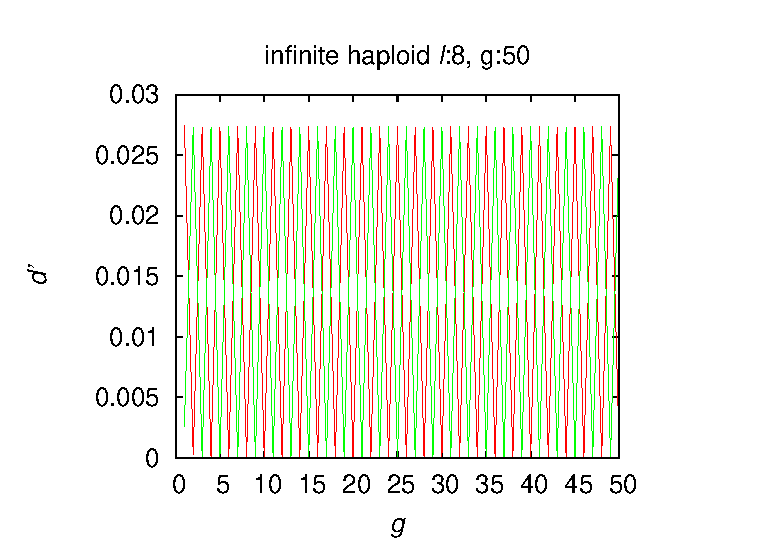
\includegraphics{figures/eps/osc/b8/osc_inf_hap.eps}}} \hspace{-3em}%
\subfloat{
\resizebox{8cm}{5cm}{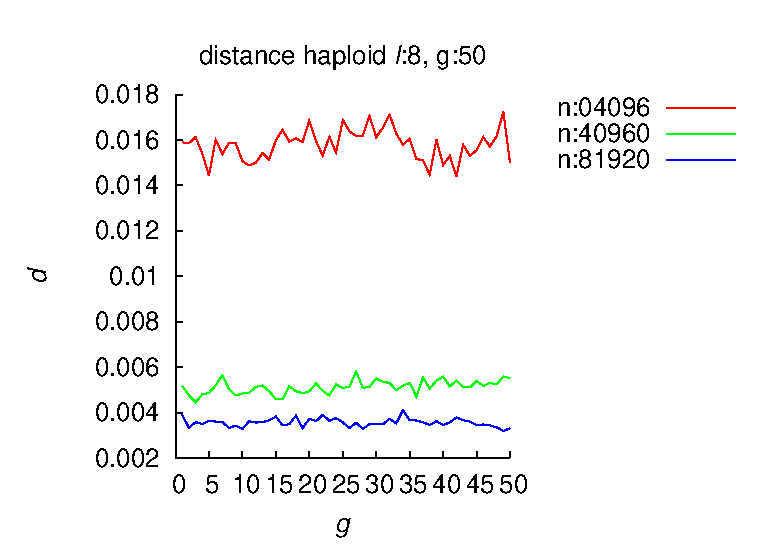
\includegraphics{figures/eps/osc/b8/fin_hap_dist.eps}}} \vspace{-0.5em} \hspace{-3em}%

\caption{\textbf{Infinite and finite haploid population oscillation behavior for genome length $\ell = 8$ (bits):} In left column, $d'$ is
  distance of finite population of size $n$ or infinite population to limits for $g$ generations. In right column, $d$ is 
  distance of finite population to infinite population for $g$ generations and $d_{avg}$ is average distances.}
\label{oscillation_8h}
\end{center}
\end{figure}

% l = 10

\begin{figure}[htp]

\begin{center}
\subfloat{
\resizebox{8cm}{5cm}{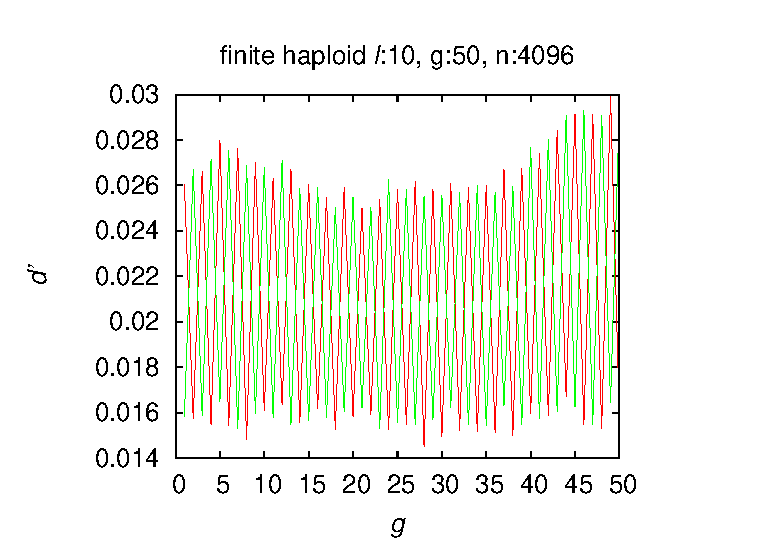
\includegraphics{figures/eps/osc/b10/n004096_osc_fin_hap.eps}}} \hspace{-3em}% 
\subfloat{
\resizebox{8cm}{5cm}{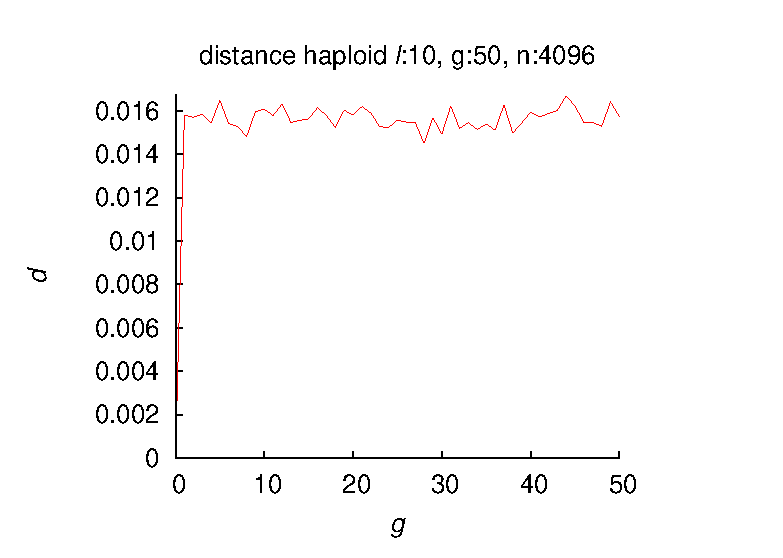
\includegraphics{figures/eps/osc/b10/n004096_osc_fin_hap_dist.eps}}} \vspace{-1em}  \hspace{-3em}% 
\end{center}
\begin{center}
\subfloat{
\resizebox{8cm}{5cm}{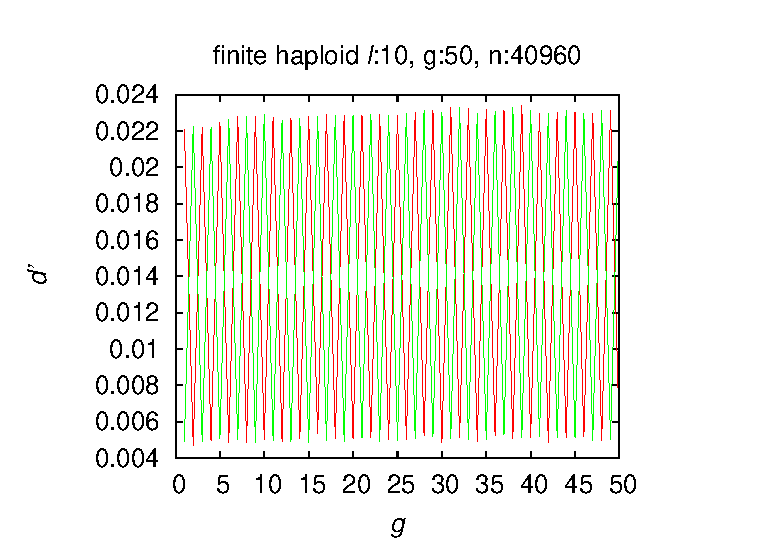
\includegraphics{figures/eps/osc/b10/n040960_osc_fin_hap.eps}}} \hspace{-3em}% 
\subfloat{
\resizebox{8cm}{5cm}{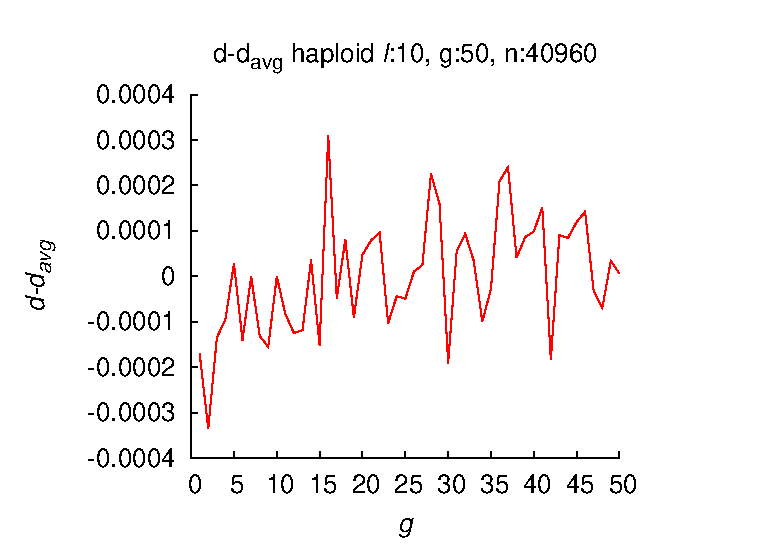
\includegraphics{figures/eps/osc/b10/n040960_osc_fin_hap_dist.eps}}} \vspace{-1em}  \hspace{-3em}% 
\end{center}

\begin{center}
\subfloat{
\resizebox{8cm}{5cm}{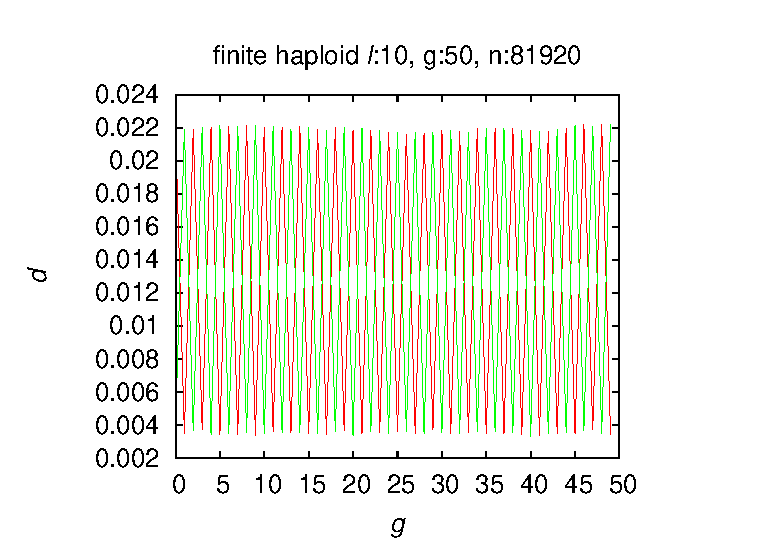
\includegraphics{figures/eps/osc/b10/n081920_osc_fin_hap.eps}}} \hspace{-3em}% 
\subfloat{
\resizebox{8cm}{5cm}{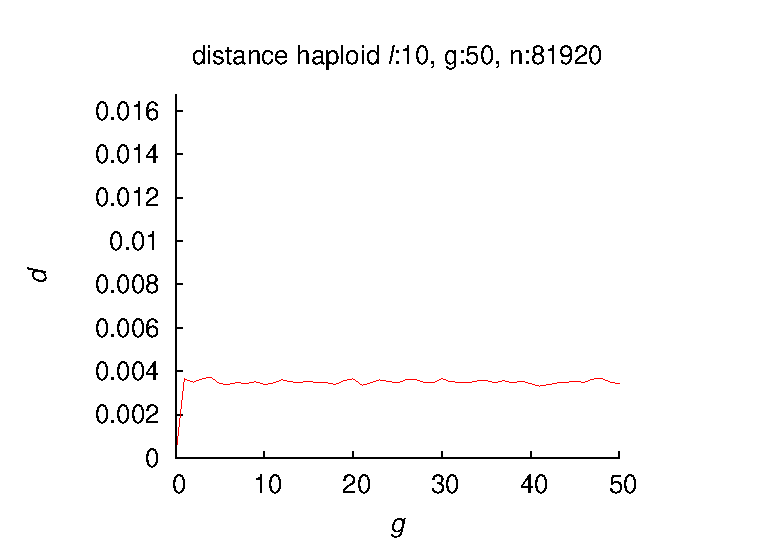
\includegraphics{figures/eps/osc/b10/n081920_osc_fin_hap_dist.eps}}} \vspace{-1em}  \hspace{-3em}% 
\end{center}

\begin{center}
\subfloat{
\resizebox{8cm}{5cm}{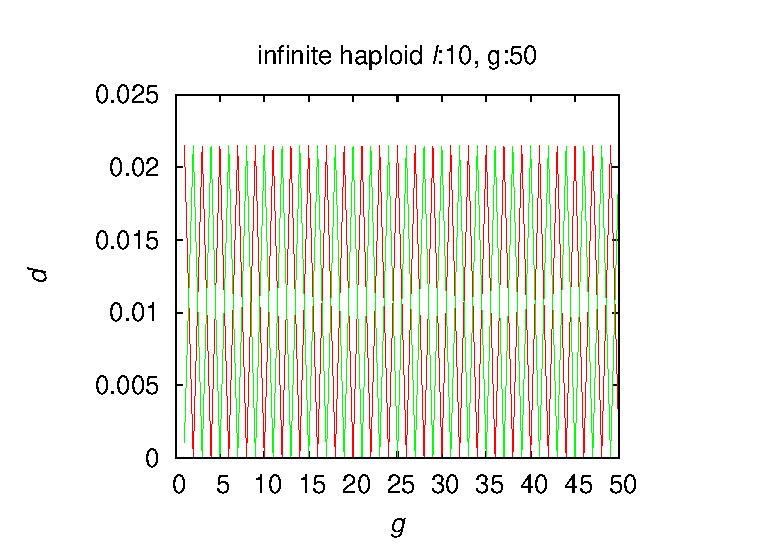
\includegraphics{figures/eps/osc/b10/osc_inf_hap.eps}}} \hspace{-3em}%
\subfloat{
\resizebox{8cm}{5cm}{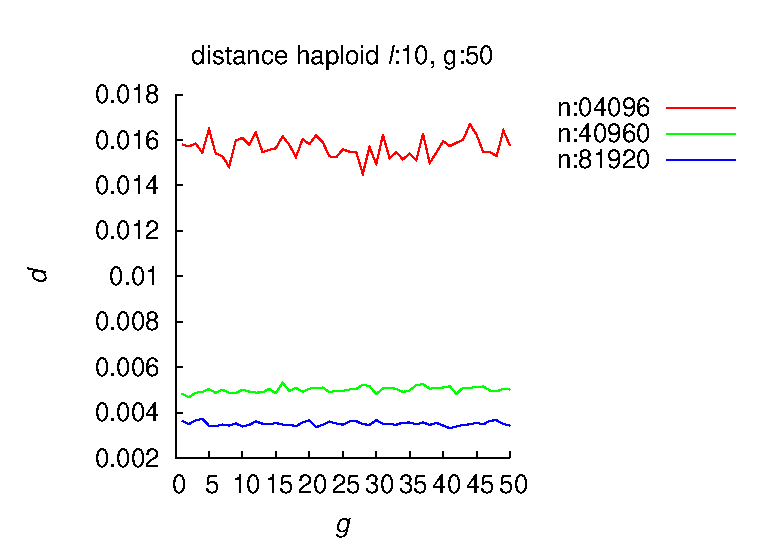
\includegraphics{figures/eps/osc/b10/fin_hap_dist.eps}}} \vspace{-0.5em} \hspace{-3em}%

\caption{\textbf{Infinite and finite haploid population oscillation behavior for genome length $\ell = 10$ (bits):} In left column, $d'$ is
  distance of finite population of size $n$ or infinite population to limits for $g$ generations. In right column, $d$ is 
  distance of finite population to infinite population for $g$ generations and $d_{avg}$ is average distances..}
\label{oscillation_10h}
\end{center}
\end{figure}

% l = 12

\begin{figure}[htp]

\begin{center}
\subfloat{
\resizebox{8cm}{5cm}{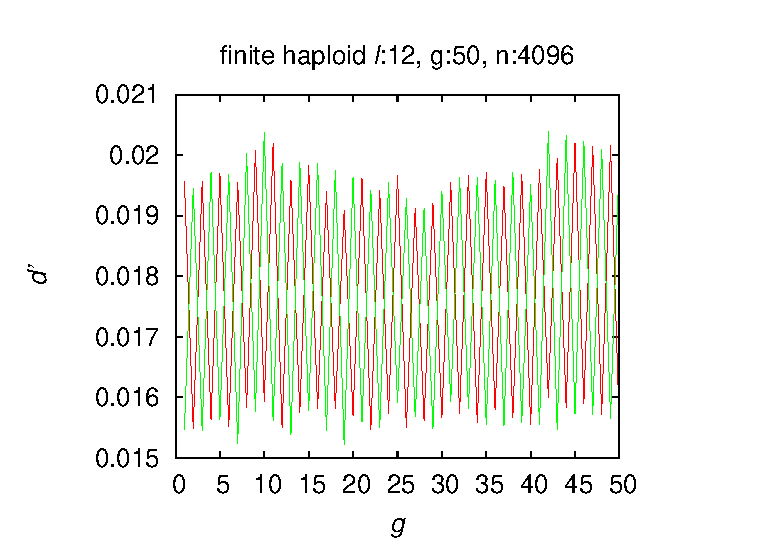
\includegraphics{figures/eps/osc/b12/n004096_osc_fin_hap.eps}}} \hspace{-3em}% 
\subfloat{
\resizebox{8cm}{5cm}{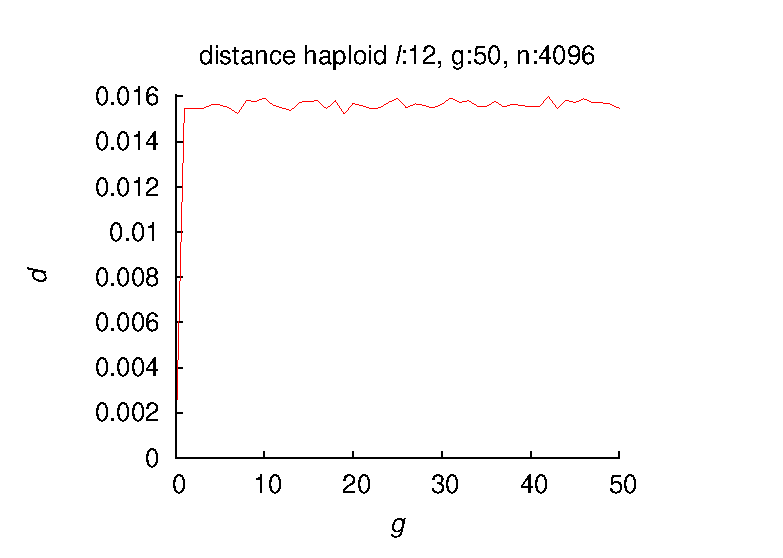
\includegraphics{figures/eps/osc/b12/n004096_osc_fin_hap_dist.eps}}} \vspace{-1em}  \hspace{-3em}% 
\end{center}
\begin{center}
\subfloat{
\resizebox{8cm}{5cm}{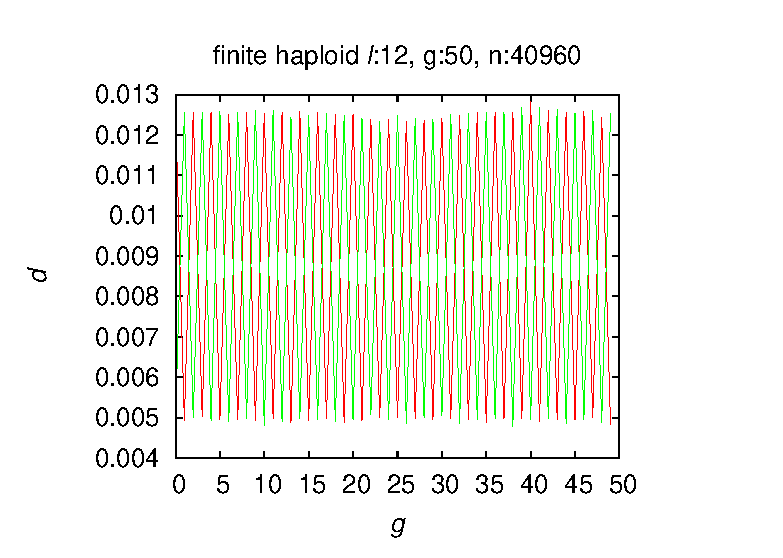
\includegraphics{figures/eps/osc/b12/n040960_osc_fin_hap.eps}}} \hspace{-3em}% 
\subfloat{
\resizebox{8cm}{5cm}{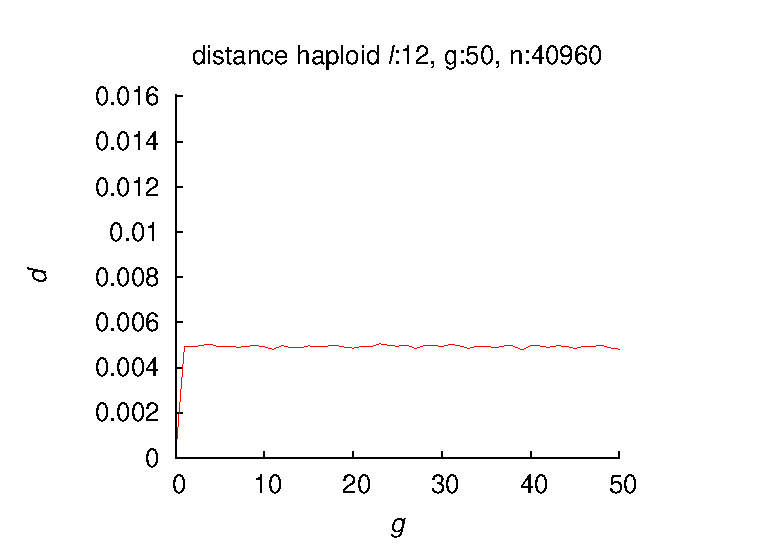
\includegraphics{figures/eps/osc/b12/n040960_osc_fin_hap_dist.eps}}} \vspace{-1em}  \hspace{-3em}% 
\end{center}
\begin{center}
\subfloat{
\resizebox{8cm}{5cm}{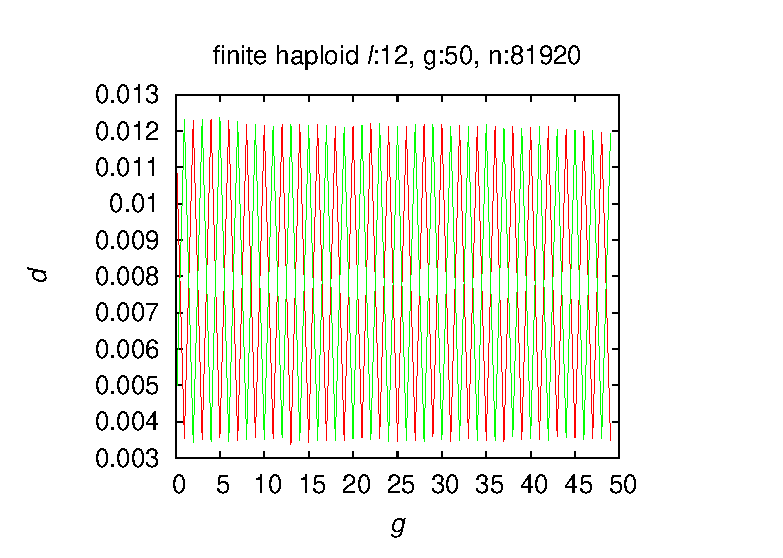
\includegraphics{figures/eps/osc/b12/n081920_osc_fin_hap.eps}}} \hspace{-3em}% 
\subfloat{
\resizebox{8cm}{5cm}{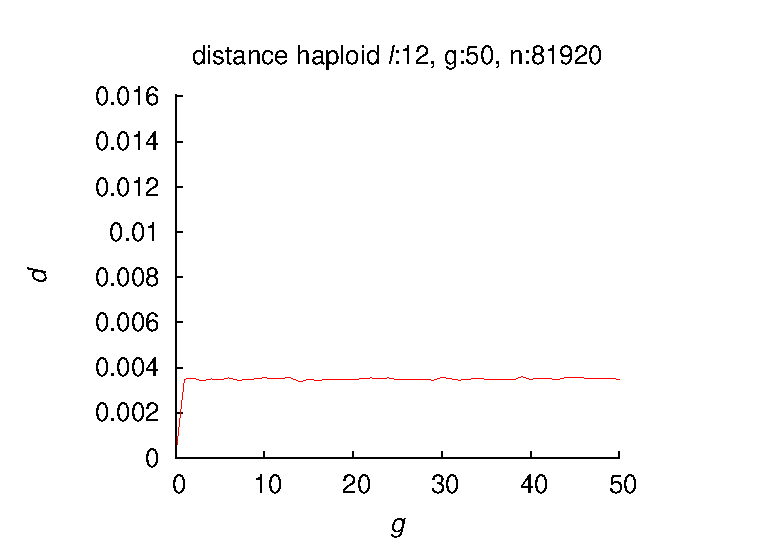
\includegraphics{figures/eps/osc/b12/n081920_osc_fin_hap_dist.eps}}} \vspace{-1em}  \hspace{-3em}% 
\end{center}

\begin{center}
\subfloat{
\resizebox{8cm}{5cm}{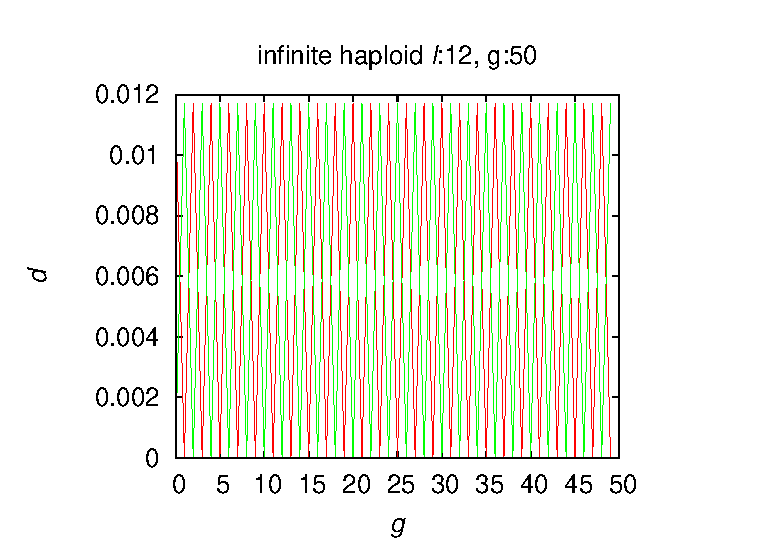
\includegraphics{figures/eps/osc/b12/osc_inf_hap.eps}}} \hspace{-3em}%
\subfloat{
\resizebox{8cm}{5cm}{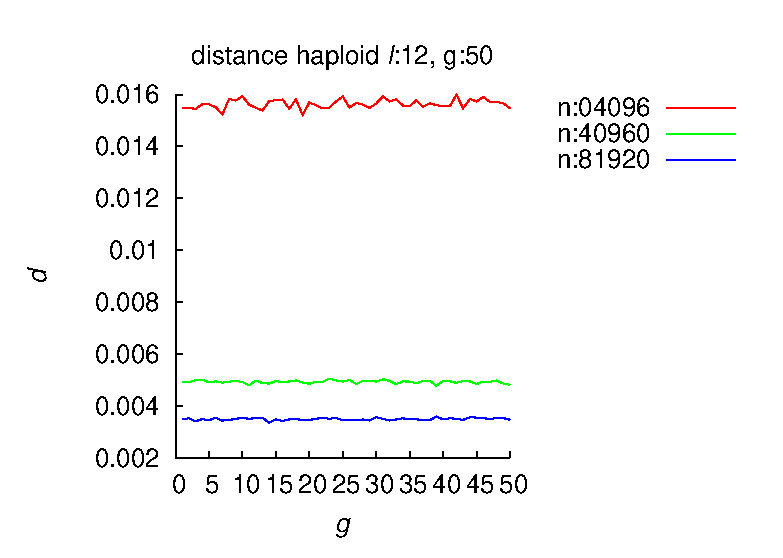
\includegraphics{figures/eps/osc/b12/fin_hap_dist.eps}}} \vspace{-0.5em} \hspace{-3em}%

\caption{\textbf{Infinite and finite haploid population oscillation behavior for genome length $\ell = 12$ (bits):} In left column, $d'$ is
  distance of finite population of size $n$ or infinite population to limits for $g$ generations. In right column, $d$ is 
  distance of finite population to infinite population for $g$ generations and $d_{avg}$ is average distances..}
\label{oscillation_12h}
\end{center}
\end{figure}

% l= 14

\begin{figure}[htp]

\begin{center}
\subfloat{
\resizebox{8cm}{5cm}{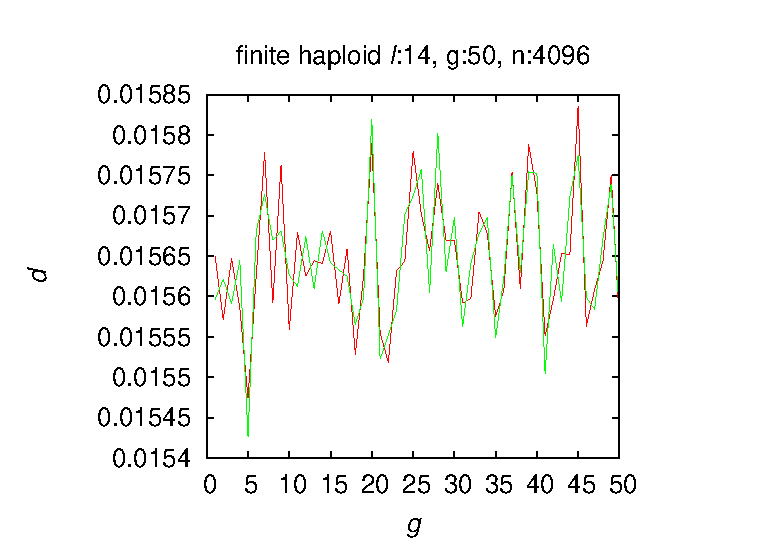
\includegraphics{figures/eps/osc/b14/n004096_osc_fin_hap.eps}}} \hspace{-3em}% 
\subfloat{
\resizebox{8cm}{5cm}{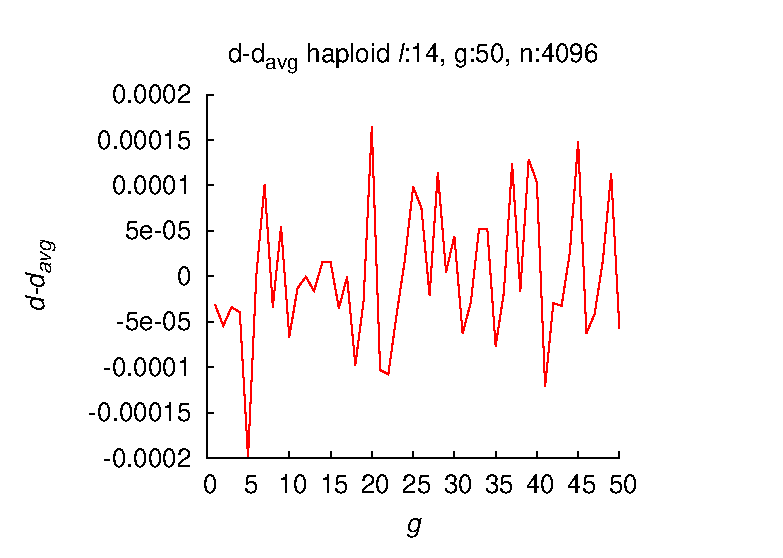
\includegraphics{figures/eps/osc/b14/n004096_osc_fin_hap_dist.eps}}} \vspace{-1em}  \hspace{-3em}% 
\end{center}
\begin{center}
\subfloat{
\resizebox{8cm}{5cm}{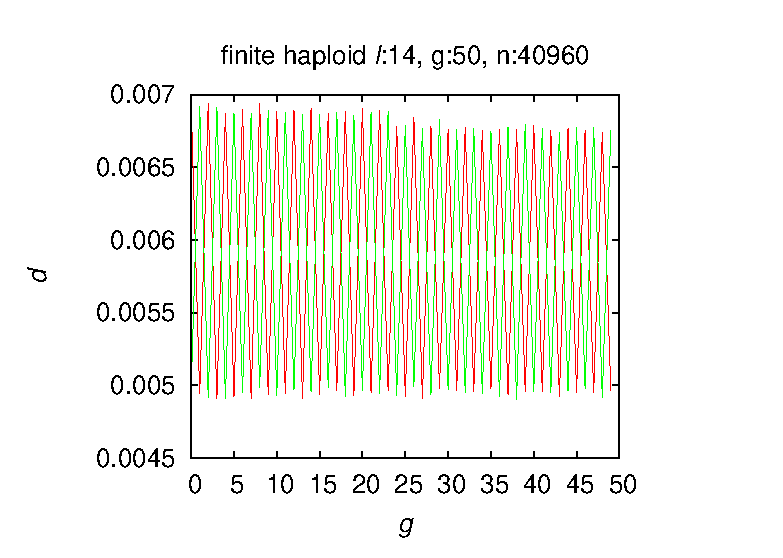
\includegraphics{figures/eps/osc/b14/n040960_osc_fin_hap.eps}}} \hspace{-3em}% 
\subfloat{
\resizebox{8cm}{5cm}{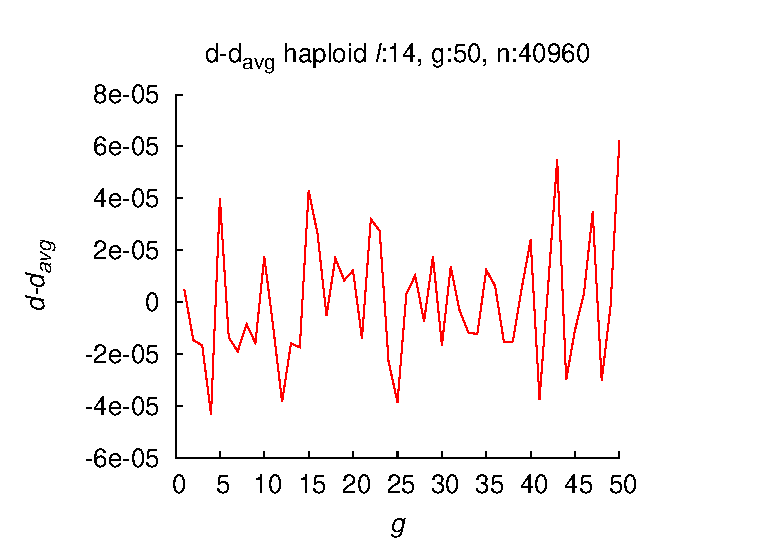
\includegraphics{figures/eps/osc/b14/n040960_osc_fin_hap_dist.eps}}} \vspace{-1em}  \hspace{-3em}% 
\end{center}

\begin{center}
\subfloat{
\resizebox{8cm}{5cm}{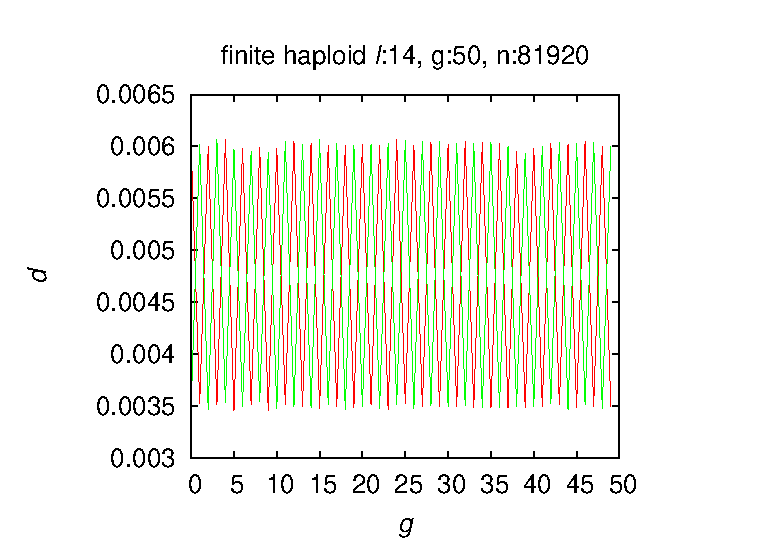
\includegraphics{figures/eps/osc/b14/n081920_osc_fin_hap.eps}}} \hspace{-3em}% 
\subfloat{
\resizebox{8cm}{5cm}{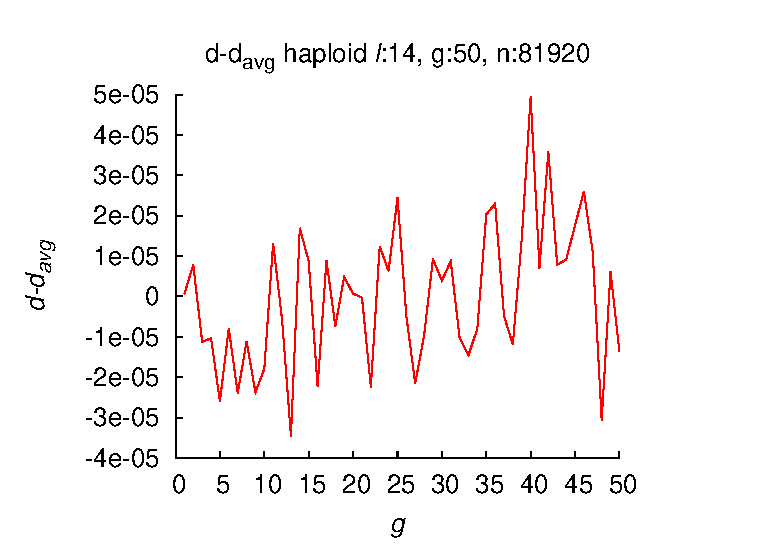
\includegraphics{figures/eps/osc/b14/n081920_osc_fin_hap_dist.eps}}} \vspace{-1em}  \hspace{-3em}% 
\end{center}

\begin{center}
\subfloat{
\resizebox{8cm}{5cm}{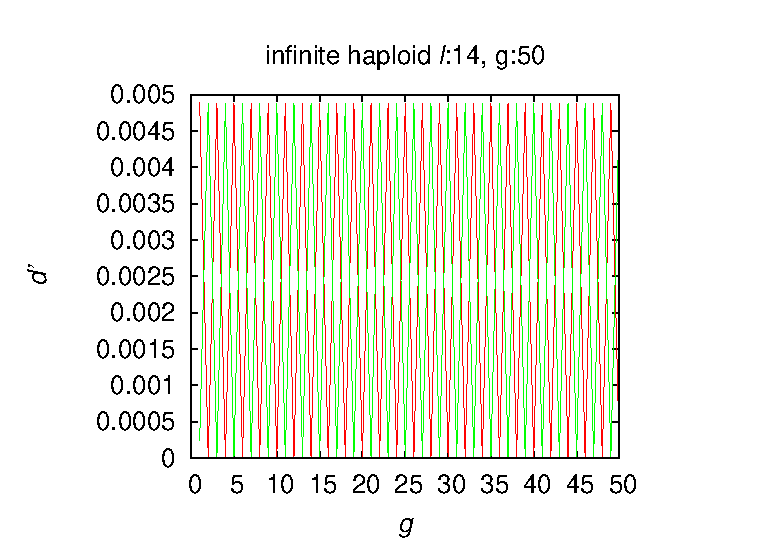
\includegraphics{figures/eps/osc/b14/osc_inf_hap.eps}}} \hspace{-3em}%
\subfloat{
\resizebox{8cm}{5cm}{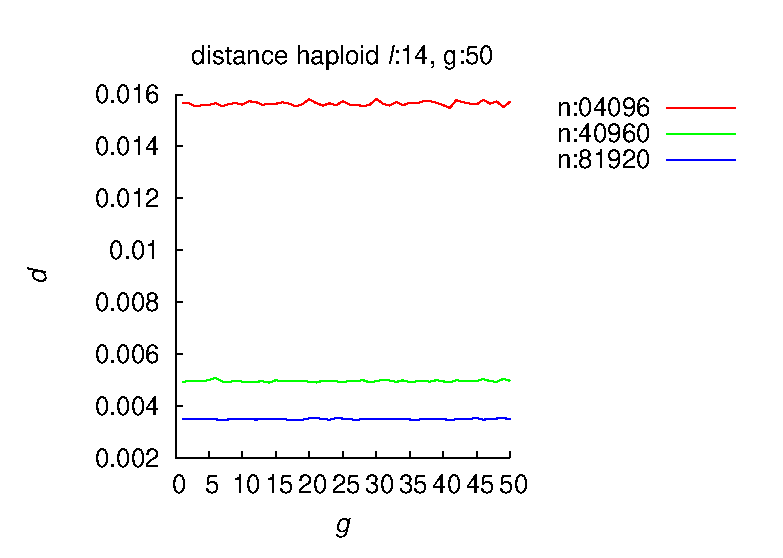
\includegraphics{figures/eps/osc/b14/fin_hap_dist.eps}}} \vspace{-0.5em} \hspace{-3em}%

\caption{\textbf{Infinite and finite haploid population oscillation behavior for genome length $\ell = 14$ (bits):} In left column, $d'$ is
  distance of finite population of size $n$ or infinite population to limits for $g$ generations. In right column, $d$ is 
  distance of finite population to infinite population for $g$ generations and $d_{avg}$ is average distances..}
\label{oscillation_14h}
\end{center}
\end{figure}

%oscillation